\documentclass[10pt,twocolumn,letterpaper]{article}
\usepackage[T1]{fontenc}
\usepackage[pagenumbers]{cvpr}
\usepackage{microtype}
\definecolor{cvprblue}{rgb}{0.16,0.30,0.50}
\usepackage[breaklinks,colorlinks,allcolors=cvprblue]{hyperref}
\graphicspath{{../results/figures/}}
\newcommand{\NyuAbsRel}{0.11455}
\newcommand{\NyuRMSE}{0.39889}
\newcommand{\NyuDelta}{0.89222}
\newcommand{\StereoMAE}{1.895}
\newcommand{\StereoCoverage}{75.69}
\newcommand{\TemporalGain}{18.23}
\newcommand{\EdgeRetention}{97.58}
\newcommand{\OriginalFPS}{2.77}
\newcommand{\EfficientFPS}{4.34}
\newcommand{\SpeedGain}{56.9}
\newcommand{\EfficientGain}{16.82}
\newcommand{\EfficientEdge}{97.64}

\def\confName{CVPR}
\def\confYear{2027}
\title{Flow-Guided Fusion for Stable Relative Depth:\\An Independent Small-Model Study}
\author{Eugene\\HKUST (Guangzhou)\\AIAA 3201 Computer Vision Project}
\date{}
\begin{document}
\maketitle
\begin{abstract}
Monocular depth can look geometrically plausible while changing across frames. We independently reproduce the revised course baselines and study a causal, training-free temporal improvement. StereoSGBM on 15 Middlebury quarter-resolution pairs obtains \StereoMAE{} pixels mean disparity error at \StereoCoverage\% mean valid coverage. RGB-only UniDepthV2 ViT-S obtains AbsRel \NyuAbsRel{}, RMSE \NyuRMSE{} m, and $\delta_1=\NyuDelta$ on all 654 NYU test images under the specified course protocol, without scale fitting. For relative video depth, we align the previous fused prediction using Farneback flow, reject inconsistent correspondences, and gate history using photometric and depth agreement. A configuration selected on a separate development clip reduces a fixed-support temporal proxy by \TemporalGain\% on rollercoaster while retaining \EdgeRetention\% of baseline edge strength. Stronger smoothing ablations lose boundaries and respond slowly to controlled depth changes. A separately disclosed engineering follow-up increases median full-pipeline throughput from \OriginalFPS{} to \EfficientFPS{} FPS. These video findings concern stability rather than metric accuracy. The official linked rollercoaster asset contains only 70 frames, so the requested 100-frame deliverable remains provisional. Code and reproducible results: \url{https://github.com/Lingxiaolingqc/MMDEVC/tree/feat/independent-direction-a/independent}.
\end{abstract}

\section{Introduction}
An RGB camera supplies appearance but no direct distance measurement. Stereo recovers distance from calibrated correspondences, while a pretrained monocular model uses learned visual regularities. Both can fail at boundaries and ambiguous surfaces. Video adds another problem: independently plausible predictions can change between adjacent frames.

Consider aligned relative predictions of 10 and 12 for one surface. Averaging may reduce noise, but unaligned history can mix different objects, newly revealed pixels have no historical support, and real depth changes make old predictions stale. Stability must therefore be evaluated alongside responsiveness.

We separate geometry, metric-image evaluation, and relative-depth video comparison as the revised assignment requires. Official Small pretrained networks remain frozen. Our independent contribution is validated data handling, evaluation, causal fusion, controlled ablations, an application, and experiment records.

We ask whether confidence fusion preserves boundaries better than simpler smoothing, and what it costs on a laptop GPU. A frozen prediction can score zero change while being wrong, so the smallest temporal residual is not automatically the best output.

\paragraph{Scope and source discrepancy.}
The linked official video has 70 decodable frames at $960\times540$, 24 FPS; its SHA-256 begins \texttt{7268cbec}. We process all genuine frames without exported duplication or interpolation. A longer course source or TA clarification is required before claiming the requested 100-frame compliance.

\section{Related Work}
Semi-global matching connects correspondence costs to calibrated stereo distance~\cite{hirschmuller2008}. Middlebury exposes thin structures and difficult matches~\cite{scharstein2014}. KITTI is a major outdoor benchmark~\cite{geiger2012}, but is not required by the revised scope.

DPT uses transformers for dense prediction~\cite{ranftl2021}; Depth Anything and DA V2 improve relative-depth representations~\cite{yang2024da,yang2024dav2}. Our unchanged frame-wise baseline is DA V2-Small, whose scores are not meters.

UniDepth/UniDepthV2 and Depth Pro address metric depth~\cite{piccinelli2024,piccinelli2025,bochkovskii2025}. We retain UniDepthV2 ViT-S's official RGB-only inference and evaluate its raw meter-valued outputs on the NYU split~\cite{silberman2012}.

RAFT is a learned optical-flow approach~\cite{teed2020}; we use CPU Farneback flow with forward/backward checks. VDA-Small provides an offline temporal reference~\cite{chen2025}, under a different operating condition from our causal method. Optional RGB-D datasets such as TUM~\cite{sturm2012} could provide further geometric validation, but were not used.

\section{Method}
\begin{figure*}[t]
\centering
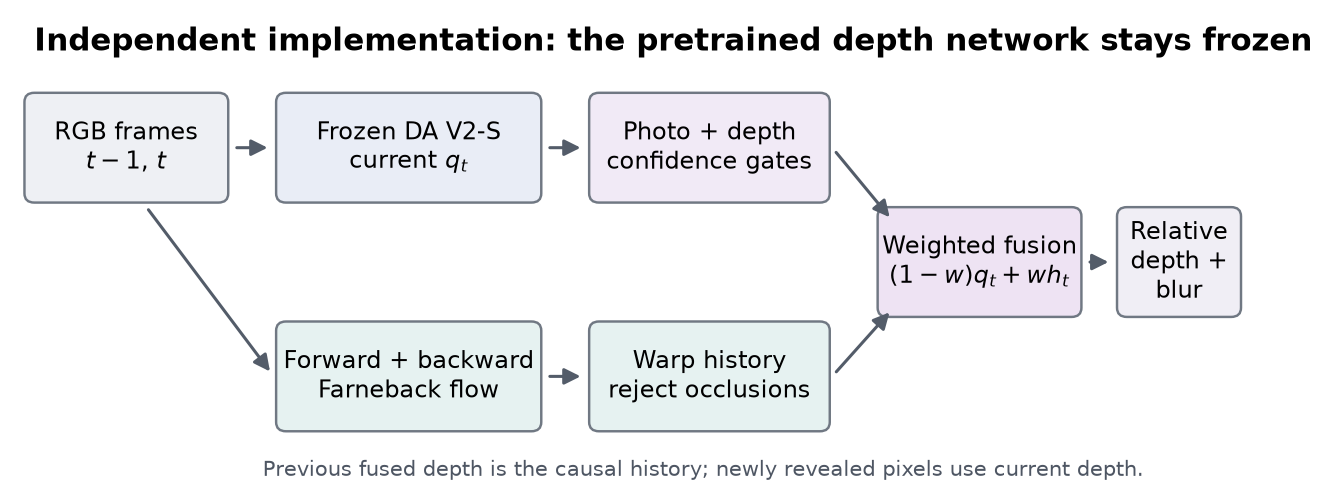
\includegraphics[width=\textwidth]{pipeline.png}
\caption{Our causal flow-guided pipeline. The depth network is frozen. Historical predictions are gathered in current-frame coordinates; unsupported or inconsistent pixels receive no history. The recurrent state is the previous fused map, so it can carry older information without consuming future RGB frames.}
\label{fig:pipeline}
\end{figure*}

\subsection{Classical and Pretrained Baselines}
StereoSGBM returns fixed-point disparity. If its raw output is $r$, pixel disparity is $d=r/16$. For the supplied quarter-resolution calibration, depth is
\begin{equation}
z=\frac{f B}{d+\mathrm{doffs}}\frac{1}{1000},
\end{equation}
where $f$ is focal length in pixels, $B$ is the baseline in millimeters, and the final factor converts to meters. For example, $r=160$, $f=1000$, $B=100$, and $\mathrm{doffs}=2$ give $d=10$ pixels and $z=8.333$ m. Invalid disparities are excluded, not converted into artificial finite depths.

For video, let $I_t$ be the RGB frame and $q_t=F(I_t)$ the raw DA V2-Small prediction. $F$ denotes the frozen pretrained network. We use $q$ to emphasize a relative, disparity-like score rather than metric distance. Larger DA V2 scores generally correspond to nearer regions. No video ground truth or meter-valued calibration is supplied.

UniDepthV2 is evaluated separately as a metric model. We do not feed unordered NYU test images into temporal fusion. Thus the NYU numbers establish the required metric baseline; they are not claimed as an improvement from Direction A.

\subsection{Motion and Backward Sampling}
Let $b_t(p)$ map current pixel $p$ to its corresponding coordinate in frame $t-1$. The historical prediction is gathered as
\begin{equation}
h_t(p)=\widetilde q_{t-1}\bigl(p+b_t(p)\bigr),
\end{equation}
using bilinear interpolation, where $\widetilde q$ is the fused recurrent state. This is destination-to-source sampling. Passing forward flow directly into this gather would reverse the correspondence.

In a one-dimensional example, a feature moves from old coordinate 2 to current coordinate 3. Its backward displacement is $-1$, so current coordinate 3 reads old coordinate 2. A request for old coordinate $-1$ falls outside the image and must be invalid. We test identity, integer translation, fractional interpolation, border handling, and non-finite input explicitly.

Flow is stored in pixel units at the output resolution. When a flow field is resized, its horizontal and vertical components are multiplied by the actual width and height ratios. For instance, resizing from $2\times3$ to $6\times6$ maps displacement $(1,1)$ to $(2,3)$. This matters in the later efficiency study.

\subsection{Occlusion and Confidence}
Forward flow $f_{t-1}$ should approximately undo the backward displacement:
\begin{align}
e_t(p)&=\left\|b_t(p)+f_{t-1}(p+b_t(p))\right\|^2,\\
m_t(p)&=\left\|b_t(p)\right\|^2+
\left\|f_{t-1}(p+b_t(p))\right\|^2.
\end{align}
We accept a correspondence when it is in bounds, finite, and $e_t(p)<0.01m_t(p)+\beta$. The selected $\beta$ is $0.5$ in squared full-resolution pixel units. This is a heuristic occlusion/reliability filter, not perfect visibility estimation.

For accepted pixels, we compare the current RGB value with warped previous RGB and compare current depth with aligned history. Writing the mean RGB residual on $[0,1]$ as $r_I$ and current-frame depth interquartile range as $s_q$, confidence is
\begin{equation}
c_t=\exp(-r_I/0.1)\,
\exp\left(-|q_t-h_t|/(0.5\max(s_q,10^{-6}))\right).
\end{equation}
The photometric term discounts mismatched appearance; the depth term reduces trust in old predictions that disagree with the current observation. These are uncalibrated reliability signals. Appearance changes, poor flow, and real depth changes can all reduce confidence.

The effective history weight is $w_t=0.75\,v_t c_t$, where $v_t$ is the validity mask. The maximum weight is 0.75, but most pixels need not receive that weight. We fuse
\begin{equation}
\widetilde q_t=(1-w_t)q_t+w_t h_t.
\end{equation}
For the toy scores 10 and 12, an actual weight of 0.25 produces 10.5. If history is invalid, $w_t=0$ and the output is exactly 10. A scene cut resets history. We use a conservative mean RGB-change threshold fixed before final evaluation. Relative affine history calibration is not used.

\subsection{Controlled Ablations and Selection}
We compare the unchanged baseline, unaligned exponential moving average (EMA), fixed-weight flow fusion, flow with occlusion rejection, and adaptive fusion. Final ablations share the selected history cap; the unchanged baseline has zero history. VDA is a separately trained reference, not one of our fusion modules.

We select parameters on the first 100 Tokyo-Walk frames. Rollercoaster is reserved for the primary frozen fusion evaluation. Twelve adaptive candidates vary the history cap over $\{0.25,0.5,0.75\}$, consistency offset over $\{0.5,1.5\}$, and depth-agreement scale over $\{0.2,0.5\}$. Fixed ablations are evaluated alongside this bounded search.

Eligibility requires at least 90\% baseline-edge strength, no more than two frames to reach 90\% of a synthetic depth step, and synthetic mean-squared error no worse than 1.05 times the raw prediction. Among eligible non-baselines, we select the smallest development temporal proxy. The chosen configuration is committed before the primary rollercoaster fusion run. These constraints are engineering criteria, not ground-truth guarantees for the real clip.

\section{Data and Evaluation Protocol}
\subsection{Static Data}
We evaluate all 15 quarter-resolution Middlebury pairs. The official ZIP names their folder \texttt{trainingQ}, corresponding to the brief's \texttt{trainQ} shorthand. StereoSGBM uses block size 5, $P_1=200$, $P_2=800$, uniqueness ratio 10, speckle window 100, and \texttt{SGBM\_3WAY}. Disparity search range is the provided calibration range rounded up to a multiple of 16. These fixed settings were independently chosen without fitting to ground-truth errors.

Ground-truth support is finite, positive disparity. Prediction support additionally requires finite, positive predicted disparity. MAE is computed on their intersection, and coverage uses all valid ground-truth pixels as its denominator. We average pair-level MAE and coverage equally and also retain all support counts. The PFM header's display-scale magnitude is not multiplied into its pixel-valued disparity samples; a real-data smoke test and a dedicated regression check guard this distinction.

NYU uses the original-format labeled MAT file and official \texttt{splits.mat}. MATLAB indices are converted to zero-based Python IDs. RGB is read as \texttt{images[i].transpose(2,1,0)} and filled metric depth as \texttt{depths[i].T}. We use 795 development and all 654 disjoint test images. Mirror transport is recorded with file hashes; the MAT structure and a downloaded prefix from the university source are checked.

Predictions are resized to $480\times640$ with bilinear interpolation. Evaluation uses Python crop $[45:471,41:601]$, a $426\times560$ region. Ground truth must be finite and strictly between 0.001 and 10 m; predictions are clipped to $[0.001,10]$ m. Non-finite predictions fail the run instead of silently excluding hard pixels. We compute AbsRel, RMSE, and $\delta_1$ per image and average images equally. The $\delta_1$ ratio threshold is strictly less than 1.25. There is no scale fitting or test alignment.

\subsection{Video and Visual Controls}
Both depth models process the same genuine rollercoaster frames at the original 24 FPS. Shared RGB/output size is $640\times360$. DA V2 uses official input size 518 and FP16. VDA-Small runs offline, with its stock overlap and keyframe procedure. Internal window padding follows its official code and is trimmed back to the genuine output count; it does not create extra submitted frames.

We first run VDA at input size 518. Its reported memory exceeds the physical laptop budget in reserved CUDA memory, so our main reference uses the permitted input size 392. This choice changes the video model's internal input, not the shared displayed frames or canvas. Each model retains its required preprocessing. All fusion variants retain the unchanged DA V2 input setting.

We freeze display normalization over each complete clip using its 2nd and 98th percentiles. DA V2 and every fusion variant share the unchanged DA V2 range. VDA has its own fixed range. A common palette therefore aids comparison but does not establish common metric scale across the two models.

\subsection{Temporal and Synthetic Diagnostics}
The real clip has no depth labels. Our optional temporal proxy uses one fixed Farneback evaluator and non-occlusion mask for every candidate. We average absolute current/warped-previous differences on the same supported pixels and divide by one baseline sequence IQR. Candidate confidence cannot remove hard pixels from the evaluation mask. Support is reported.

This proxy has two limitations. Its flow family is related to the fusion backend, and flow aligns image correspondences without compensating true scalar-depth changes caused by 3D motion. We therefore do not describe its reduction as metric accuracy. Raw temporal values across clips with different content should not be compared as a universal quality scale.

We also report retained gradient strength at the unchanged baseline's strongest depth edges. This is an edge-preservation proxy, not precision/recall against true depth boundaries. Known-truth synthetic controls include independent noisy predictions, a translating foreground, newly revealed background, a real depth step, and a scene cut. A frozen-depth negative control demonstrates that zero temporal change alone can certify nothing about correctness.

\section{Results and Analysis}
\begin{table}[t]
\centering
\caption{Independent mandatory static baselines. NYU uses the course protocol and raw metric scale; stereo is a separate exercise.}
\begin{tabular}{lr}
\toprule Measurement & Result\\
\midrule Middlebury pairs & 15\\
Mean pair disparity MAE (px) & \StereoMAE\\
Mean valid coverage (\%) & \StereoCoverage\\
\midrule NYU test images & 654\\
UniDepthV2-S AbsRel & \NyuAbsRel\\
UniDepthV2-S RMSE (m) & \NyuRMSE\\
UniDepthV2-S $\delta_1$ & \NyuDelta\\
\bottomrule
\end{tabular}
\label{tab:static}
\end{table}

\begin{figure*}[t]
\centering
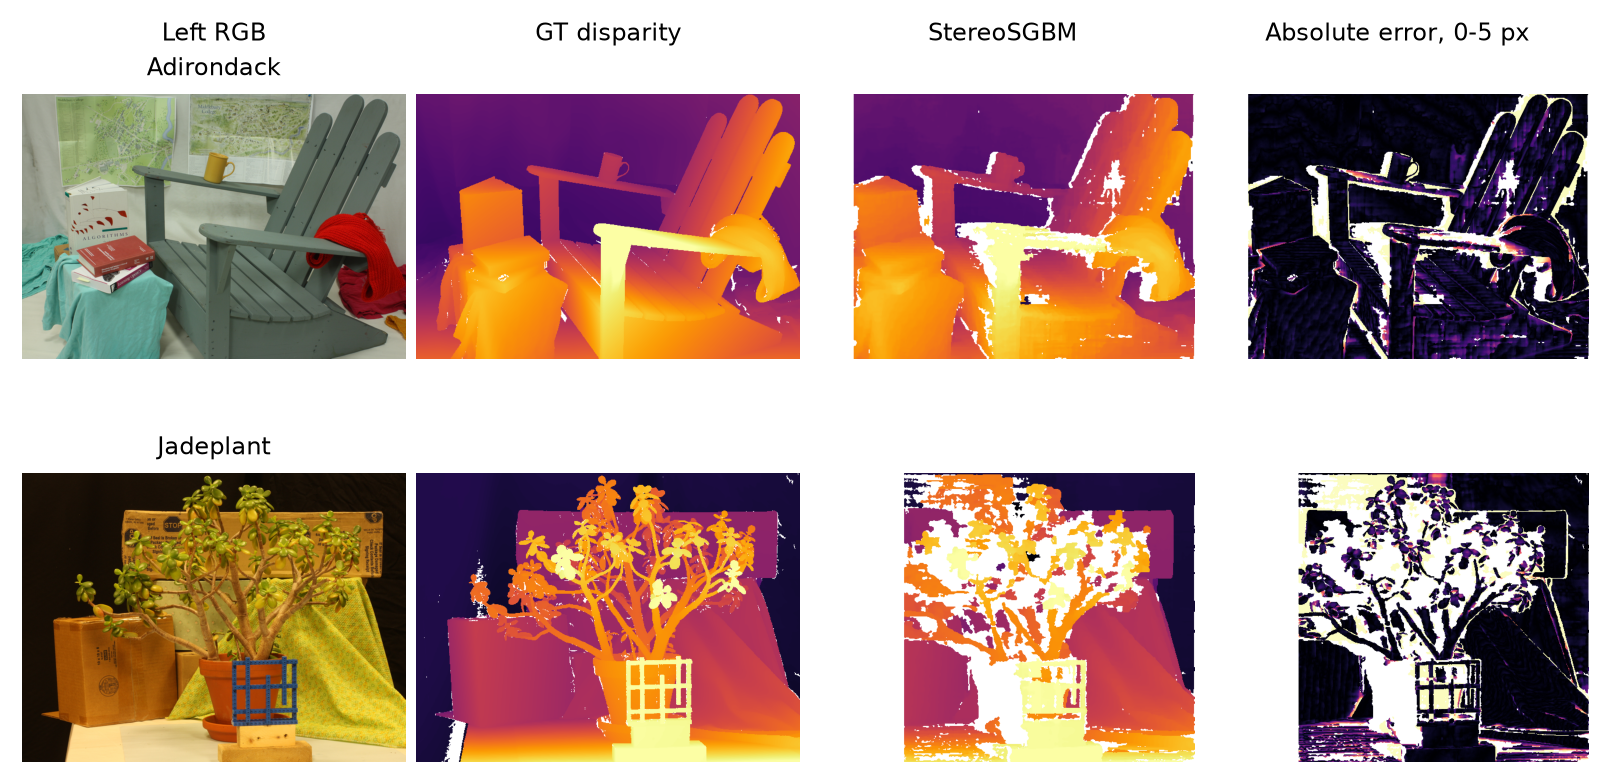
\includegraphics[width=\textwidth]{stereo-comparison.png}
\caption{Middlebury examples. Disparity colors share a fixed range within each pair; absolute error is clipped to 5 px for display only. Unsupported predictions are masked. Thin leaves and complex occlusions in Jadeplant remain more difficult than the textured surfaces in Adirondack. Coverage accompanies error so rejecting pixels cannot be mistaken for uniform accuracy.}
\label{fig:stereo}
\end{figure*}

\subsection{Static Accuracy}
Table~\ref{tab:static} reports our own runs. Stereo obtains \StereoMAE{} px MAE with \StereoCoverage\% mean valid coverage. The exercise illustrates the connection between calibration, disparity units, and valid support, rather than serving as the metric monocular benchmark. Jadeplant and PianoL have high pair-level errors, demonstrating why an aggregate alone is insufficient. Figure~\ref{fig:stereo} shows thin structures and invalid regions explicitly.

UniDepthV2-S obtains AbsRel \NyuAbsRel{}, RMSE \NyuRMSE{} m, and $\delta_1=\NyuDelta$. These are course-protocol scores, not claims of exact reproduction of a paper's benchmark number. Differences in crop, image set, resizing, precision, or metric aggregation can change the result even with the same checkpoint. The median measured official inference time is 58.37 ms/image after two warmups, excluding image I/O, metrics, and prediction compression.

\subsection{Primary Frozen Video Comparison}
\begin{figure*}[t]
\centering
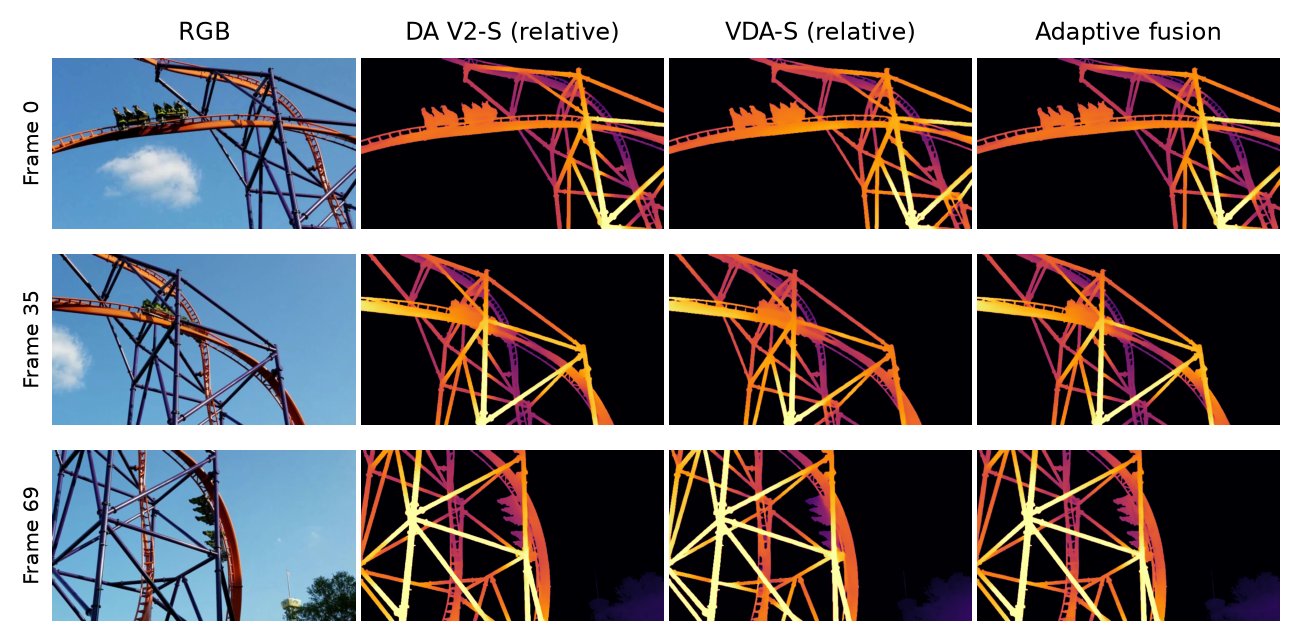
\includegraphics[width=\textwidth]{video-comparison.png}
\caption{Chronological frames 0, 35, and 69, selected for an overview rather than by performance. All displays use whole-clip ranges. Adaptive fusion shares DA V2's range; VDA uses its own, so equal colors across models do not imply equal distances. The first fused frame is identical to the baseline by initialization.}
\label{fig:video}
\end{figure*}

Table~\ref{tab:ablation} shows the main frozen evaluation. Adaptive fusion reduces the temporal proxy from 0.10797 to 0.08829, a \TemporalGain\% reduction, while retaining \EdgeRetention\% of baseline edge strength. Figure~\ref{fig:video} shows the train, thin supports, and changing view over the complete source interval. The associated videos preserve every genuine frame.

The table also makes the main tradeoff visible. Occlusion-only fusion has a much lower temporal residual, 0.03461, but retains only 79.4\% of baseline edge strength at the same history cap. A smaller residual can thus accompany substantial spatial attenuation. The synthetic depth-step response takes nine frames for these fixed-weight high-history ablations, versus one for adaptive fusion. We do not hide this result by declaring the most complex method universally best.

EMA performs particularly poorly on this moving scene: its flow-aligned proxy exceeds the unchanged baseline and only 30.3\% of edge strength remains. It averages fixed pixel locations that can correspond to different objects over time. Alignment helps, and reliability checks reduce inappropriate propagation, but strong fixed history still has a responsiveness cost.

\begin{table}[t]
\centering
\caption{Primary frozen ablations. Temporal is a baseline-IQR-normalized proxy, lower being smoother. Edge strength is relative to the unchanged prediction, not ground-truth boundary accuracy. Step settling uses synthetic truth.}
\resizebox{\columnwidth}{!}{\begin{tabular}{lrrr}
\toprule Method & Temporal & Edge (\%) & Step frames\\
\midrule
Frame-wise & 0.10797 & 100.0 & 1 \\
EMA & 0.12938 & 30.3 & 9 \\
Flow & 0.03688 & 76.6 & 9 \\
Occlusion & 0.03461 & 79.4 & 9 \\
Adaptive (selected) & 0.08829 & 97.6 & 1 \\
\bottomrule
\end{tabular}
}
\label{tab:ablation}
\end{table}

\begin{figure*}[t]
\centering
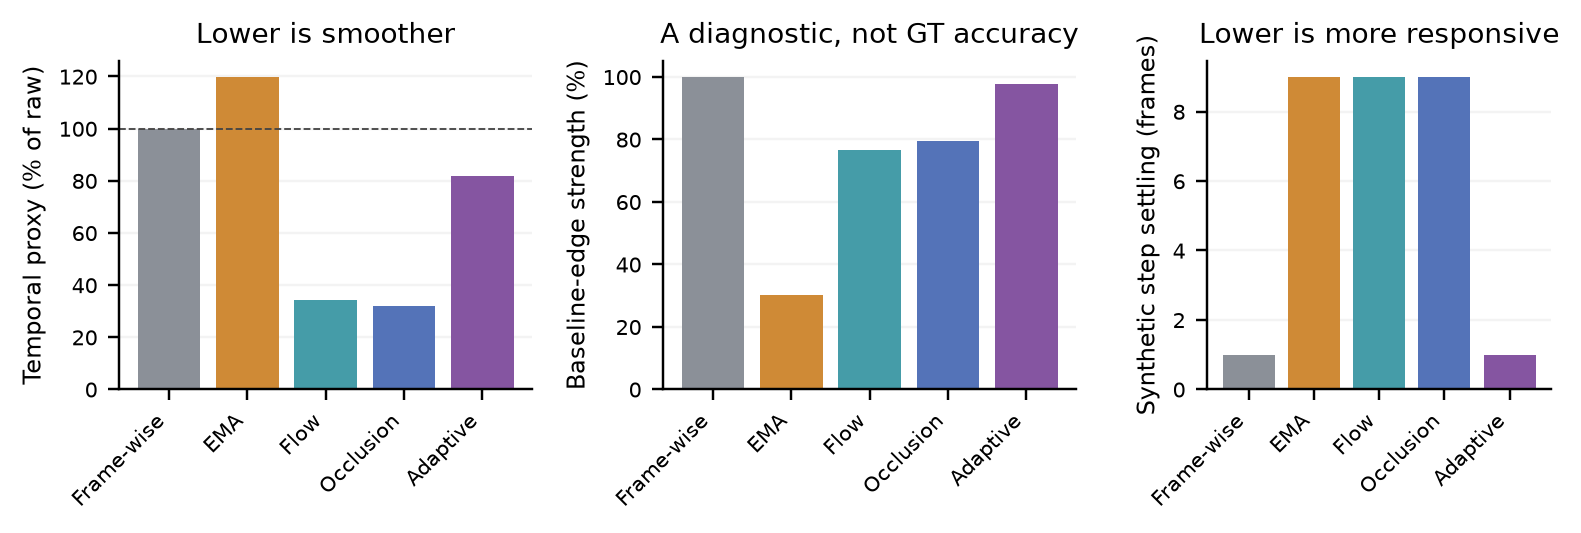
\includegraphics[width=\textwidth]{ablations.png}
\caption{Stability, edge retention, and synthetic responsiveness must be read together. Fixed-weight smoothing can minimize temporal change while attenuating boundaries or delaying a true depth step. Adaptive fusion gives up some smoothing to preserve the current observation.}
\label{fig:tradeoff}
\end{figure*}

\subsection{Why the Confidence Gate Helps}
The depth-disagreement gate allows the current frame to dominate when history diverges sharply. In the synthetic step, the RGB frame can remain unchanged while depth changes, so photometric matching alone would not detect stale history. Conversely, RGB disagreement can identify correspondence problems even when two relative predictions have similar scalar values. Neither signal is a calibrated uncertainty model, but together they reduce uncritical reuse of historical predictions.

The selected development setting reduces the Tokyo proxy from 0.01032 to 0.00593, retaining 94.7\% of baseline edge strength. Its synthetic noisy-motion MSE is 0.07988, compared with 0.09080 for unchanged predictions. These development findings motivate the frozen choice; they are not substituted for held-out evidence.

Thin supports and the moving train in Figure~\ref{fig:video} make history sensitive to alignment and visibility. Adaptive fusion stays closer to current boundaries than aggressive smoothing, but without depth labels a retained edge is not necessarily physically correct.

\begin{figure*}[t]
\centering
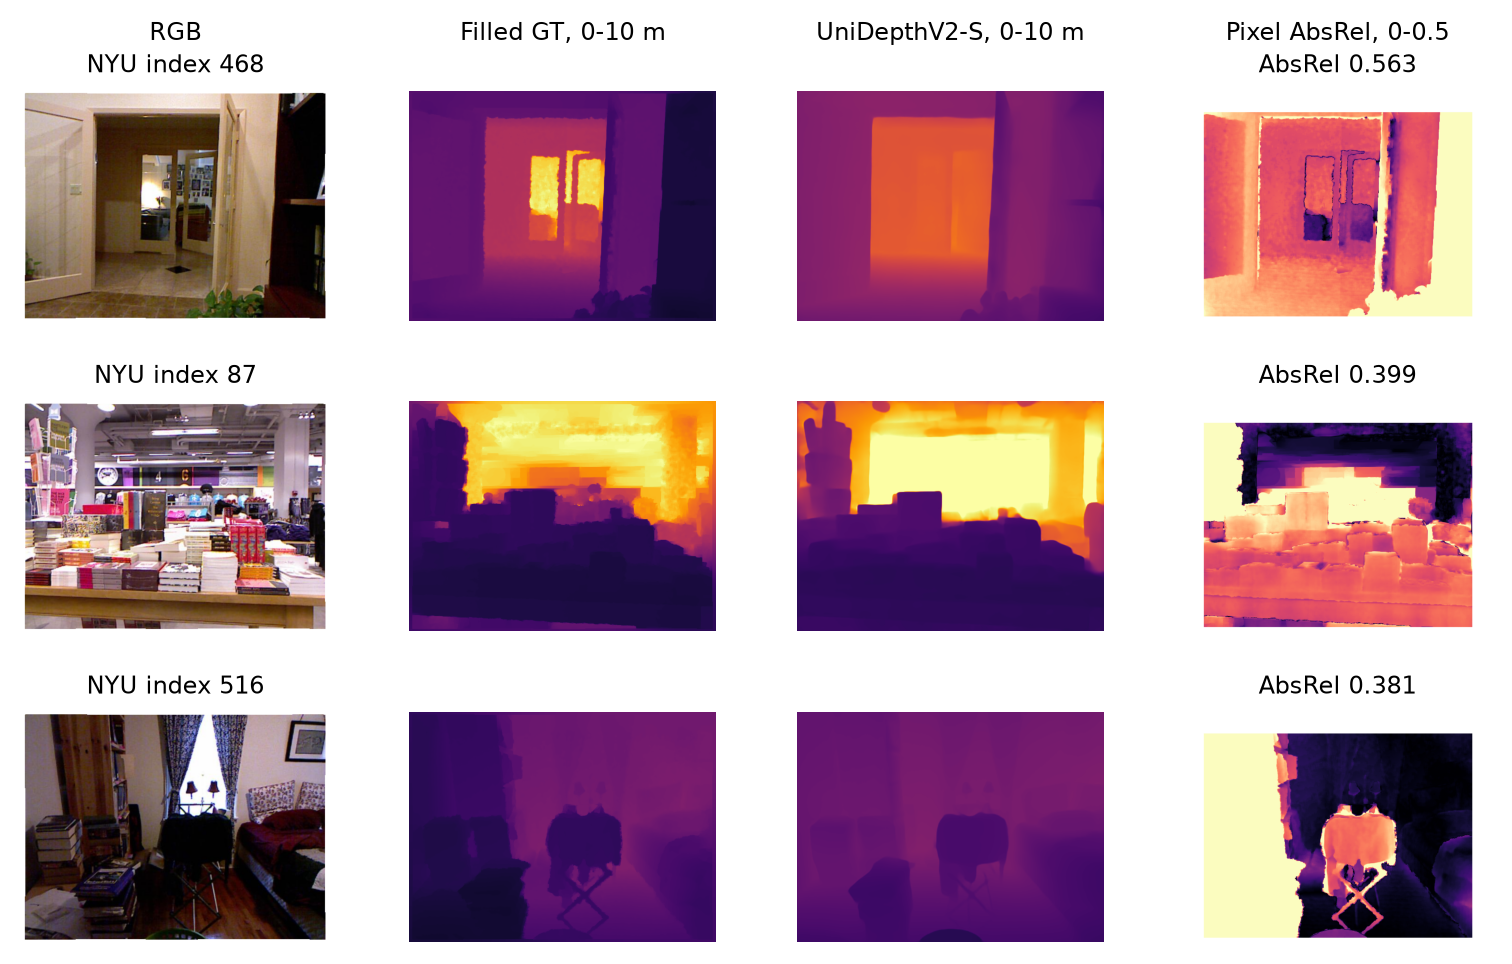
\includegraphics[width=\textwidth]{nyu-failures.png}
\caption{The three NYU images with highest measured test AbsRel, selected automatically. Doorway/interior depth, cluttered shop layers, and thin chair geometry near a bright window remain difficult. GT and prediction share 0--10 m colors. Pixel AbsRel is shown only on the evaluation crop and capped at 0.5 for display. Filled ground truth also has limitations.}
\label{fig:failures}
\end{figure*}

\subsection{Efficiency and a Disclosed Engineering Follow-up}
Experiments use an RTX 4070 Laptop GPU with 8,188 MiB VRAM, Python 3.12.6, PyTorch 2.8.0/CUDA 12.8, and OpenCV 4.11.0.86. Depth uses FP16 where supported; flow/fusion use float32. Networks run sequentially.

Three synchronized trials measure actual DA V2 inference, both flow directions, and fusion. These trials recompute predictions and flow; cached ablation replay is not reported as full-pipeline FPS. RGB decode/resize and disk video encoding are excluded and named separately in run records. The original setting achieves median \OriginalFPS{} FPS, with trial range 2.61--2.92 FPS. Peak allocated CUDA memory for this pipeline is approximately 386 MiB, since optical flow is CPU-based.

Profiling identifies flow as the main cost. A separate engineering study therefore compares flow widths 320, 480, and 640 on development data only. We choose the smallest width whose development proxy is within 5\% of the original and whose edge-strength retention is at least 90\%. Width 320 qualifies: 0.00612 versus 0.00593 at width 640, with 94.9\% edge retention. Displacements are rescaled back to full output coordinates; the evaluator remains fixed at width 640.

The secondary efficient setting achieves median \EfficientFPS{} FPS, \SpeedGain\% faster than the original, while its secondary rollercoaster evaluation retains an \EfficientGain\% proxy reduction and \EfficientEdge\% edge strength. We preserve the original result as the primary frozen test. This follow-up occurred after the first held-out evaluation; although its setting was selected solely on development data, we label its final score as a later engineering experiment rather than a fresh untouched test.

VDA-Small at input size 518 takes 73.49 s for 70 frames with 8,014 MiB peak allocated and 11,858 MiB reserved. The permitted size 392 takes 6.94 s with 3,072 MiB allocated and 4,194 MiB reserved; we use this reference. Windows logical CUDA counters do not prove physical residency. Timing depends on hardware and operating conditions; these are local measurements.

\subsection{Metric Failure Cases and Application}
Figure~\ref{fig:failures} deliberately shows the three worst per-image AbsRel cases, rather than visually attractive successes. Image 468 has a doorway and strongly differing interior depth interpretation; image 87 contains densely layered shop objects and large scale errors; image 516 contains a thin chair and bright window boundaries. Their per-image AbsRel values are 0.563, 0.399, and 0.381. The selection rule and IDs are saved so the cases can be reproduced.

These failures distinguish convincing shape from correct metric scale. Relative video fusion does not repair a separate metric model's calibration. Future RGB-D validation could help separate model errors from ambiguous filled labels.

Our depth-aware background blur normalizes with the unchanged depth range and blends RGB with a Gaussian-blurred image using a fixed focus threshold and transition. Baseline and fused inputs share all settings. The side-by-side demo exposes mask bleeding and lag at moving boundaries; its focus threshold is relative, not a physical distance.

\section{Reproducibility, Limitations, and Contribution}
Source, tests, configurations, per-image/per-pair summaries, and figures reside in a separate directory and feature branch. Large inputs/caches stay outside Git. Records retain upstream/model/data identities, frame IDs, settings, and timing scope; the primary configuration was committed before fusion evaluation.

Early runs predated automatic source hashing; missing hashes are not invented retrospectively. New runs capture Git/dirty state, source/config hashes, environment, and lockfile identity. Tests cover metrics, data axes/units, warping, synthetic behavior, fixed support, rendering, and archive claims.

The 70-frame source cannot meet the literal 100-frame requirement without external clarification. Packaging requires provisional mode and a warning. Real-video depth and poses are unavailable: flow residuals can penalize genuine depth changes, and edge retention can preserve noise. Synthetic controls simplify real motion, lighting, and occlusion. Recursive errors may accumulate on longer clips. One development clip cannot establish robustness to exposure changes or difficult flow.

Our contribution is fusion/evaluation code and analysis. Official architectures, training, weights, and inference remain attributed. Worked examples support learning; AI-assisted creation alone is not evidence of student mastery.

\section{Conclusion}
Confidence fusion reduces the primary temporal proxy by \TemporalGain\% with \EdgeRetention\% edge retention and better responsiveness than aggressive smoothing. A separate development-selected flow study increases throughput from \OriginalFPS{} to \EfficientFPS{} FPS. Static baselines use explicit units and masks. Less temporal change alone does not establish better depth. The demo remains provisional pending resolution of the source-length discrepancy.

\clearpage
{\small
\bibliographystyle{ieeenat_fullname}
\bibliography{references}
}
\end{document}
